\section{Daily measurement definitions}
\label{app:daily}

\subsection{Feasibility and coverage}

Feasibility is assessed for each branch and measurement family before aggregation. A derivable quantity is supported within a stated retained population; this designation does not imply continuous acquisition or applicability to every service offered by the protocol. A quantity requiring additional acquisition has a plausible source or linkage requirement. Inapplicable quantities do not describe the sampled unit, whereas unknown quantities lack sufficient evidence to resolve their status. Figure~\ref{fig:feasibility} summarizes selected families; the accompanying matrix includes the full definitions and qualifications.
\begin{figure}[!htbp]
\centering
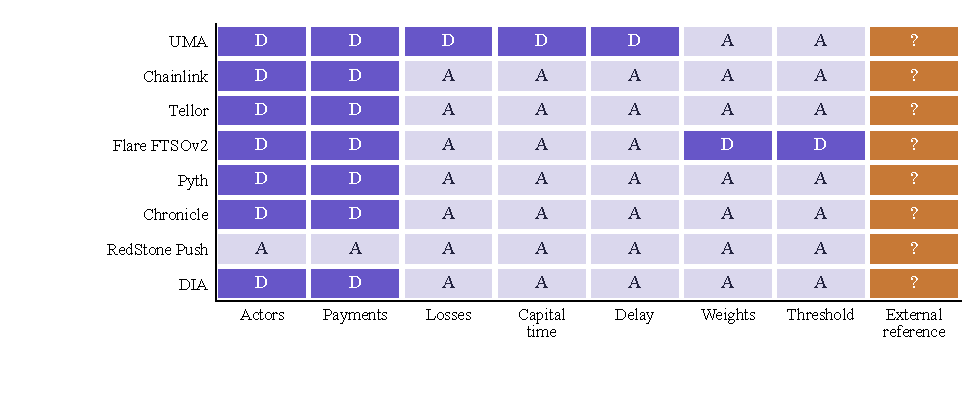
\includegraphics[width=0.99\linewidth]{figures/feasibility_gallery.pdf}
\caption{Measurement feasibility by branch. D: derivable in the retained population; A: additional acquisition or linkage needed; dash: inapplicable; question mark: unresolved. Flare weights and thresholds retain epoch support. RedStone Push covers delivery contracts; publisher participation and AVS economics require separate evidence. }
\label{fig:feasibility}
\end{figure}

\subsection{Aggregation and denominators}

For an eligible event population $\mathcal E_g$ with grouping key $g$, a daily amount is
\begin{equation}
 A_{dg}=\sum_{i\in\mathcal E_g:\,t_i\in[d,d+1)}a_i .
\end{equation}
The grouping key retains branch, implementation, actor role, asset and stage. Integer amounts are summed before decimal conversion. Eligible retained events define the denominator without establishing complete acquisition. Untimed observations cannot enter daily groups and remain in the missingness accounting.

Participation counts distinct observed addresses within a specified role. Delivery-contract activity in RedStone is recorded as contract activity, and Flare reward owners are distinguished from registered providers. Reward inequality uses positive observed recipient totals within the same day, asset and stage. The top-decile share includes the largest $\lceil0.1n\rceil$ recipient totals. A recipient with no recorded payment is outside that recipient population; its absence is not a verified zero reward.

UMA completion delay is measured from the request event to the settlement event and grouped by settlement day. Its denominator consists of completed, flow-reconciled requests. A completion fraction would additionally require a defined obligation and a comparable risk set, so it is not inferred by dividing daily settlements by daily requests. Escrow exposure is computed from the running balance implied by the request's token movements. A request is included only when its lifecycle transactions map unambiguously to that request, all included transfers are timed, balances remain nonnegative and the closing balance is zero. With balance $b_{ik}$ held between successive transfer times $t_{ik}$ and $t_{i,k+1}$, daily exposure is
\begin{equation}
 K_{di}=\sum_k b_{ik}\,\bigl|[t_{ik},t_{i,k+1})\cap[d,d+1)\bigr| .
\end{equation}
The stored quantity uses raw token-seconds; conversion to token-hours divides by the asset precision and 3,600. Fees cease contributing when they leave escrow, while funded rewards contribute for as long as they remain held. The resulting measure describes observed contract balances for the eligible closed-request cohort. It does not establish participant wealth, total protocol collateral or the amount subject to slashing.

\subsection{Historical signing policies}

Flare epoch artifacts record signers, integer weights, a threshold and the starting voting round, matched to retained voter registrations. Normalized weights $w_i$ give concentration $H=\sum_i w_i^2$ and effective address count $1/H$. The table reports the fewest largest-weight addresses needed to reach or exceed the threshold under weak and strict conventions. An operative security threshold requires historical contract and runtime evidence. These address-level measures do not identify owners, independent organizations or attack feasibility.

Entitlements, signing weights and deposited capital retain different units and roles. Epoch values keep their support intervals; uniform daily allocation does not turn reward factors into payments. Signatures and aggregate agreement do not independently measure price accuracy.

\subsection{Temporal sensitivity and lifecycle follow-up}

Weekly aggregation preserves daily event counts and integer amounts within each typed group. A separate comparison restricts observations to the intersection of the branches' retained calendar envelopes. This restriction aligns the outer dates but cannot establish continuous coverage within them. Estimates requiring verified complete intervals therefore remain unavailable. For epoch entitlements, an allocation comparison contrasts the epoch-end label with proportional overlap across UTC days. These are alternative representations of the same entitlement; neither is included among observed daily payments.

UMA follow-up retains settled and unresolved requests until settlement or the common cutoff. Figure~\ref{fig:uma_followup} shows completed-request delays and unresolved shares by request year. Delays are conditional on settlement, and cohorts have unequal follow-up. Neither panel estimates protocol-wide timely-resolution probabilities.
\begin{figure}[!htbp]
\centering
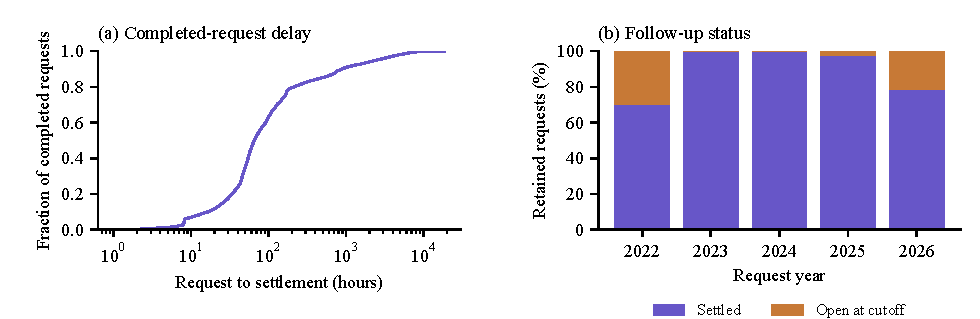
\includegraphics[width=0.99\linewidth]{figures/uma_followup.pdf}
\caption{UMA request follow-up. (a) Empirical cumulative distribution of elapsed request-event to settlement time among completed requests. (b) Settlement status at the common cutoff, grouped by the year of the request event. Requests still open at the cutoff are right-censored; an unobserved later settlement is not classified as failure.}
\label{fig:uma_followup}
\end{figure}
